% Niveau :      PCSI *
% Discipline :  Chimie Orga
% Mots clés :   IR

\begin{exercise}{Spectre infrarouge des cétones cycliques}{3}{PCSI}
{Chimie organique I,Spectroscopie,Infrarouge}{bermu}

\begin{questions}
    \questioncours Spectroscopie infrarouge.
\begin{itemize}
    \item allure d'un spectre IR ;
    \item mesure d'un spectre IR ;
    \item fonctionnement de l'appareil (grandes lignes) ;
    \item paramètres influençant la vibration d'une liason donnée (\emph{e.g.} C=O) ;
\end{itemize}
    \question Interprétez les différences observées dans les spectres des différentes cétones ci-dessous :
\end{questions}
\noindent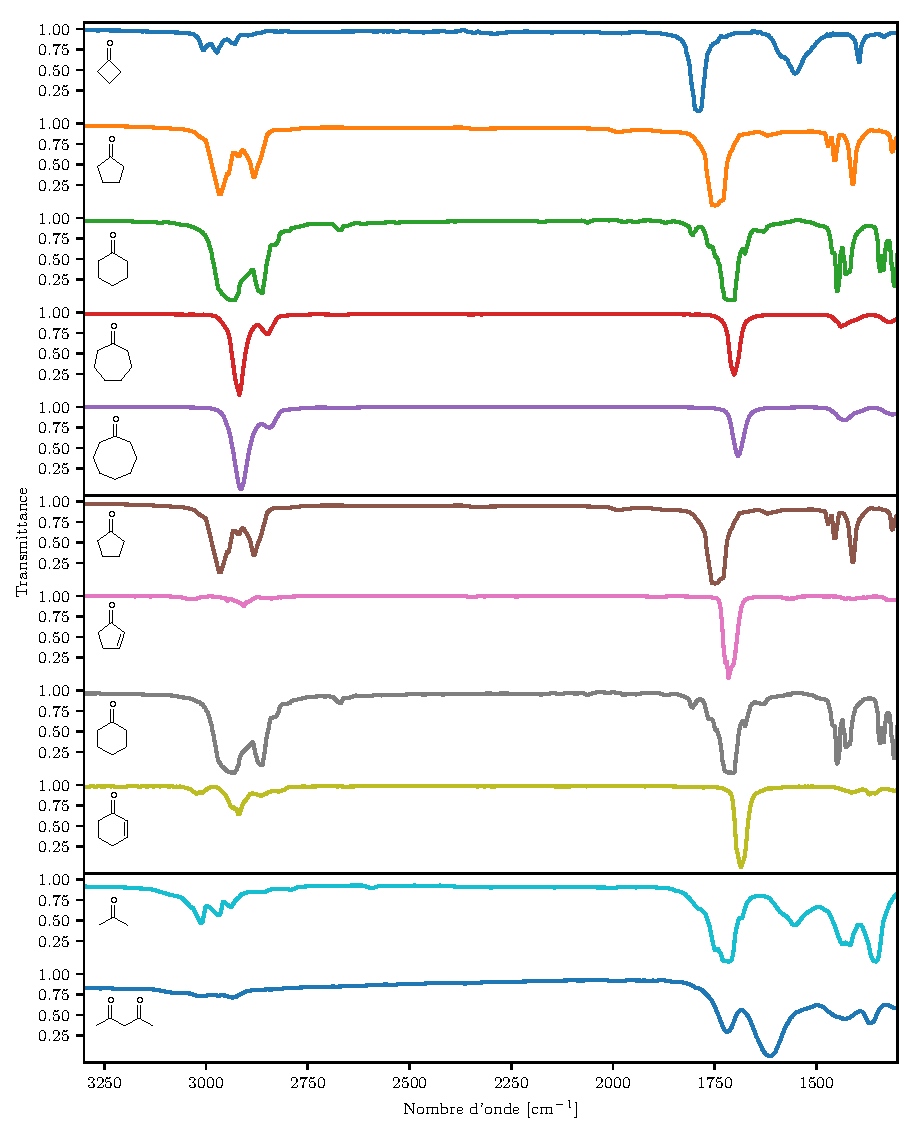
\includegraphics[width=\linewidth]{chimiePC/orga/cetones_ir_fig.pdf}
\end{exercise}